\documentclass{article}
\usepackage{siunitx} 
\usepackage{graphicx}
\usepackage{natbib}
\usepackage{amsmath} 

\setlength\parindent{0pt}

\renewcommand{\labelenumi}{\alph{enumi}.}

%\usepackage{times} 

%----------------------------------------------------------------------------------------
%	DOCUMENT INFORMATION
%----------------------------------------------------------------------------------------

\title{Práctica 5 \\ Programación Concurrente y de Tiempo Real \\Universidad de Cádiz} % Title

\author{Alejandro Serrano Fernández} % Author name

\date{\today} % Date for the report

\begin{document}

\maketitle % Insert the title, author and date


%----------------------------------------------------------------------------------------
%	SECTION 1
%----------------------------------------------------------------------------------------
\section{Ejercicio 4}
Para calcular el tiempo que tarda mi computadora en calcular resaltado de una imagen, cabe destacar que los siguientes datos han sido obtenidos a través de un portátil equipado con un i7-7700hq de 4 núcleos y 8 threads. Como podemos observar para este problema, a medida que aumentamos el número de hilos, el speedUp disminuye, esto significa que para un mayor número de hilos, el tiempo de ejecución aumenta. Los resultados obtenidos han sido los siguientes: (x = hilos, y = speedup).

\hfill \break
\begin{center}
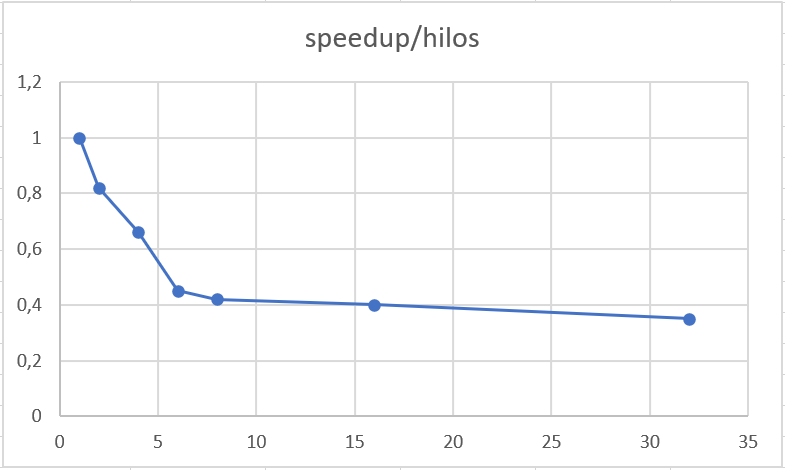
\includegraphics[scale=0.5]{grafico-ejercicio4.png}
\end{center}
Para este problema, podemos concluir que es preferible elegir la solución secuencial antes que la paralela, pues es notablemente más rápida que una solución paralela.
\end{document}



